% begin module root-functions
\begin{frame}
\begin{itemize}
\item<1->  If $n$ is a positive integer, the function $f(x) = x^{\frac{1}{n}} = \sqrt[n]{x}$ is called a root function.
\item<2->  When $n = 2$, it is the square root function $f(x) = \sqrt{x}$.
\item<3->  In this course, the square root is not defined for negative numbers, so its domain is $[0, \infty)$.
\item<4->  Its graph is the top half of the parabola $x = y^2$.
\item<5->  The graph of the cube root function $f(x) = \sqrt[3]{x}$ is similar to that of the square root, but it is defined for all real numbers.
\end{itemize}
\begin{tabular}{cc}
\uncover<2->{%
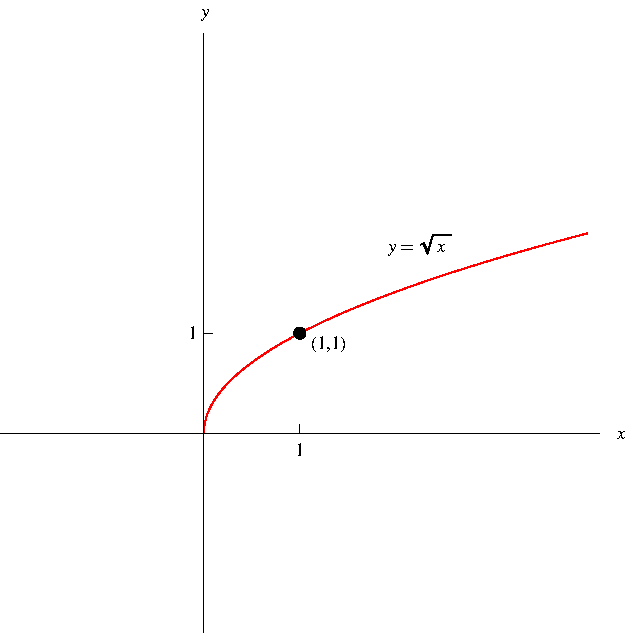
\includegraphics[height=3.5cm]{precalculus/pictures/01-02-sqrtx.pdf}%
}%
&%
\uncover<5->{%
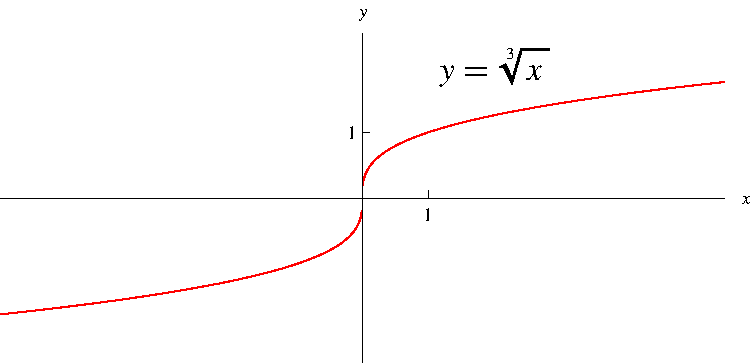
\includegraphics[height=3.5cm]{precalculus/pictures/cube-root.pdf}%
}%
\end{tabular}
\end{frame}
% end module root-functions
